\subsection{Results of Planning}
A large part of the first phase of the project (i.e. scheduling and draft) is reflected on %TODO *in?
the functional specification document. The requirement analysis is registered, the objectives are declared, whereas the decisions and the product information is written down.

\subsubsection{Software Development Model}

This section contains information about the software model chosen, based on the requirements of the project.
The principals of the group, client requirements and knowledge about the project play an important role in choosing the development model. Based on the latter, the development team decides its work flow. 

\begin{aims}
	\leftskip=0,8cm
	\item[Agile Development Model: SCRUM] The group chose SCRUM because it is an iterative and incremental agile software development framework for managing product development. The duration of each sprint was set to two weeks. Each phase of the software development has two sprints. 
	
	Every sprint ends with a presentation by the relevant %TODO the relevant working group? was soll das bedeuten?
	 working group about the developments and progress during the sprint. The end of the respective phase of the project is marked by a working prototype and a presentation which includes a summary of the work done by the entire team. 
	
	\item[Projects specific adaptation to the model:] Every person in the team has multiple roles. All group members work on both the documents and the code.
\end{aims} 

\paragraph{Software Development Specific Content}
Since the group decided for an agile development model, the milestones need to be stated and agreed upon by the team. Milestones are the aim or the expected output of each development phase. They help the team to specify what features should be completed by which deadline.

\newpage

\subsubsection{Effort Estimate}
The main purpose of the effort estimate section is the categorization of the different parts of the project regarding their complexity and effort criteria.  
 (see figure 1)

\begin{figure}[h]
	\begin{center}
		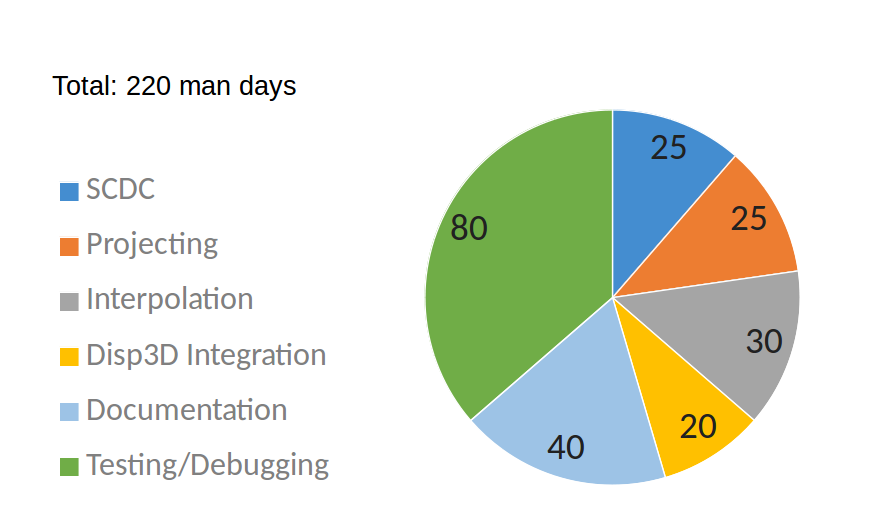
\includegraphics[width= 14cm]{figures/aufwandsabschaetzung.png}
		\caption{Effort estimate}
	\end{center}
\end{figure}

\clearpage

\subsubsection{Risk Estimate}
In this section, the probabilities of different risks involved in the project are listed. This will help the team to determine what aspects of the implementation should get a higher priority.

\begin{description}
	\item[RE1:] Communication problems in the team
	\item[RE2:] Coverage is too extensive
	\item[RE3:] Framework does not provide the needed functionality 
	\item[RE4:] Resource bottleneck deriving from team members temporary absence 
	\item[RE5:] Change of requirements due to miscommunication with the product owner 
	\item[RE6:] Hidden complexity 
	\item[RE7:] Acceptable computation time takes a lot more effort than expected  
\end{description}

\begin{figure}[h]
	\begin{center}
		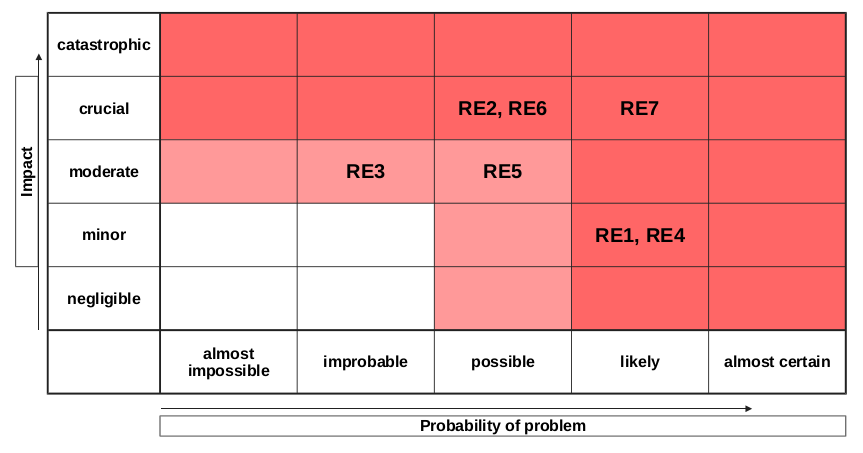
\includegraphics[width= 15cm]{figures/risikoabschaetzung.png}
		\caption{Risk estimate}
	\end{center}
\end{figure}

\paragraph{Handling Risks}

In case one of the mentioned risks occurs, certain strategies for solving the issue are provided. Only the ones having crucial impact on the project are dealt with in the following section.

\begin{aims}
	
	\item[RE2:]Optional requirements will only be addressed after every mandatory criteria is fulfilled.
	\item[RE6:]The team communicates with the product owners to eradicate all ambiguities.
	\item[RE7:]To keep the computation time as low as possible, changes to the software will be tested constantly to 						   determine even minor impacts on efficiency. 	
	
\end{aims}

\clearpage

\subsubsection{Milestones} 
These Milestones provide major dates for significant events during the time of the project. Furthermore they serve as a guideline for the progress that is desired at a certain point of time.
~\\
~\\

\begin{tabular}{lll}
 	\textbf{First Phase} & 03.05.2017 & First Phase Finished\\
	\textbf{Second Phase} & 04.06.2017 & Detailed Design and Features Implemented\\
				& 08.06.2017 & Second Phase Finished\\
	\textbf{Third Phase} & 21.06.2017 & Features Tested and Optimized\\          
				& 02.07.2017 & Portation to MNE Scan\\
				& 05.07.2017 & End of Project\\
\end{tabular}

~\\

\begin{figure}[h]
	\begin{center}
		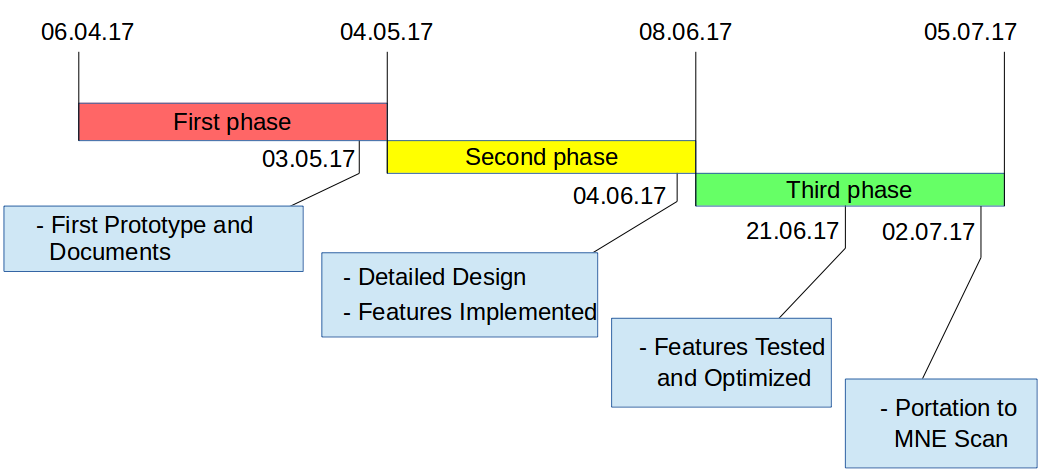
\includegraphics[width= 15cm]{figures/milestones_timeline.png}
		\caption{Timeline of milestones}
	\end{center}
\end{figure}

\paragraph{Checklist}
\begin{aims}
	\item[03.05.2017]First Phase Finished
	\begin{enumerate}\itemsep0pt 
		\item Functional Specification
		\item Preliminary Design
		\item Review Document
		\item First Prototype
		\item Presentation
	\end{enumerate}
	
	\item[04.06.2017]Detailed Design and Features Implemented
	\begin{enumerate}\itemsep0pt
		\item Detailed Design
		\item SCDC (operational)
		\item Projecting Algorithm (operational)
		\item Interpolation Algorithm (operational)
	\end{enumerate}
	
	\item[08.06.2017]Second Phase Finished
	\begin{enumerate}\itemsep0pt
		\item Presentation
		\item Review Document
		\item Integration into Disp3D
	\end{enumerate}

	\item[21.06.2017]Features Tested and Optimized
	\begin{enumerate}\itemsep0pt
		\item SCDC (tested)
		\item Projecting Algorithm (tested)
	\end{enumerate}
	
	\item[02.07.2017]Portation to MNE Scan
	
	\item[05.07.2017]End of Project
	\begin{enumerate}\itemsep0pt
		\item Review Document
		\item Presentation
		\item Interpolation Optimized
	\end{enumerate}


\end{aims}

\newpage

\subsubsection{Organization}

This section covers the rules, agreements and the partitioning regarding the teamwork in the project, so the work itself will be efficient and organized

\paragraph{Ways of Communication}
\begin{aims}
	\item[Telegram:] Used for quick and direct team communication so that possible misunderstandings will be solved in no time.
	
	\item[E-mail distribution list:] Used for scheduling the team meetings and communications with the extended team, including the product owners. 
	
	\item[Team meetings:] Used for the review and direct discussion of the encountered problems. 
	
	\item[Skype:] Used in the cases of the absence of a team member. 
	
	\item [Jira:] Used for scheduling tasks and keeping track of the progress done by each member of the team.
	
	\item[Dropbox:] Used for exchanging documents and file sharing.  
\end{aims}

\paragraph{Additional Agreements}
\begin{itemize}
	\item Internal team meetings (without product owners): Tuesdays and Thursdays at 19:00
	
	\item External team meeting (with the product owners): Wednesdays at 17:00
	
	\item Meeting of subgroups : upon consultation and demand 
\end{itemize}

\paragraph{Role Assignment in SCRUM}

\begin{aims}
	\leftskip=0,8cm
	\item[Product Owner:] Thomas Jochmann, Lorenz Esch
	
	\item[Scrum Master:] Simon Heinke
	
	\item[Development team:] Blerta Hamzallari, Felix Griesau, Julius Lerm, Lars Debor, Marco Klamke, Simon Heinke, Sugandha Sachdeva, Petros Simidyan
	
	\item[Client, User:] Participants of the MNE CPP project of Boston Children's Hospital
	
\end{aims}

\paragraph{Role Assignment Organization}
\begin{aims}
	\leftskip=0,8cm
	\item[Advisor:] Thomas Jochmann, Lorenz Esch
	
	\item[Team leader:] Simon Heinke
	
	\item[Build master:] Lars Debor
	
	\item[Version management:] Felix Griesau
	
\end{aims}

\clearpage